\chapter{Ứng dụng ma trận trong PageRank}
      
    \section{Xây dựng ma trận} 
    \subsection{Tại sao phải xây dựng ma trận?}
    Việc thực hiện xấp xỉ nghiệm bằng vòng lặp thủ công gây tốn nhiều thời gian và kém hiệu quả. Vì vậy ta cần một công cụ tốt hơn để thực hiện việc xấp xỉ nghiệm này. Và công cụ được sử dụng để tính toán trong trường hợp này là \emph{Stochastic Adjacency matrix} (ma trận xác suất chuyển đổi).
        \subsection{Stochastic Adjacency matrix - Ma trận xác suất chuyển đổi  \cite{Stochastic_Matrices}}
            Ma trận xác suất chuyển đổi là một ma trận dùng để mô tả các liên kết giữa các trang web trong một \emph{web graph}. 
            Từ \emph{web graph} ta xây dựng ma trận xác suất chuyển đổi $M$:
            \begin{itemize}
                \item Với $j$ là chỉ số dòng và $i$ là chỉ số cột.
                \item Trang thứ $i$ sẽ có $d^+(i)$ \emph{outgoing links}.
                \item $M_{ji} = \dfrac{1}{d^+(i)}$ nếu có liên kết từ trang $i$ đến trang $j$, $M_{ji} = 0$ nếu không có liên kết. Do đó tổng các cột của ma trận $M$ luôn bằng 1 \emph{(Column Stochastic matrix)}.
            \end{itemize}
         Ma trận $M$ còn có thể xây dựng bằng cách xây dựng ma trận kề $(1,0)$. Sau đó chia mỗi phần tử trong ma trận kề cho tổng giá trị của cột chứa nó. 
        \subsection{Rank vector - Vector xếp hạng}
            Với $r$ là vector có dạng $r = \{ r_1, r_2, ..., r_n\}$ với $r_i$ là giá trị đại diện cho PageRank của trang web $i$. Khi đó:$$\sum_i{r_i}  = 1.$$
        \subsection{Phương trình ma trận}
            Từ công thức tổng quát để tính PageRank của trang web, ta viết lại dưới dạng phương trình ma trận:
            $$\boxed{M \cdot r = r}$$
            
            \textbf{Ví dụ 4:} Giả sử ta có 4 trang web và liên kết như đồ thị dưới đây
            \begin{align}
                 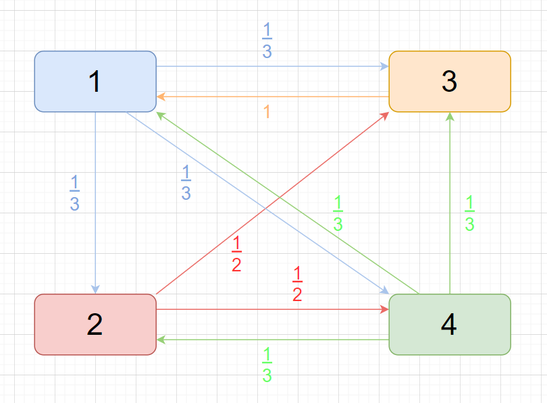
\includegraphics[width=.5\textwidth]{figure/grap1.png}
            \end{align}
            Ta tính $d^+(i)$ của từng trang web
            \begin{itemize}
                \item Trang web 1 có đường dẫn đến cả 3 trang web còn lại: $d^+(1) = \dfrac{1}{3}$
                \item Trang web 2 có đường dẫn đến trang web 3 và 4: $d^+(2) = \dfrac{1}{2}$
                \item Trang web 3 có 1 đường dẫn đến trang  web 1: $d^+(3) = 1$
                \item Trang web 4 có đường dẫn đến cả 3 trang web còn lại: $d^+(4) = \dfrac{1}{3}$
            \end{itemize}
            Ta xây dựng được ma trận $M$ sau đây: \\
            $$
            \begin{pmatrix}
                %M & 1 & 2 & 3 & 4 \\
                  0 & 0 & 1 & \dfrac{1}{3} \\[10pt]
                \dfrac{1}{3} & 0 & 0 & \dfrac{1}{3} \\[10pt]
                \dfrac{1}{3} & \dfrac{1}{2} & 0 & \dfrac{1}{3} \\[10pt]
                \dfrac{1}{3} & \dfrac{1}{2} & 0 & 0
            \end{pmatrix}
            $$

    \section{Power Iteration method - Phương pháp lũy thừa ma trận }
               
            Ta nhận thấy công thức $M \cdot r = r$ tương ứng với $Ax = \lambda x$ với $\lambda = 1$. Do đó ta nói rằng $r$ là một vector riêng của ma trận xác suất chuyển đổi $M$ ứng với trị riêng $\lambda = 1$. Cho nên ta cần phải sử dụng một phương pháp để tìm vector riêng đó đồng thời nó phải hiệu quả với ma trận $M$ có kích thước lớn.
        \subsection{Phương pháp lũy thừa ma trận là gì? \cite{Power_Iteration}}
           
         \begin{itemize}
            \item Trong thuật toán \emph{PageRank}, phương pháp lũy thừa ma trận được sử dụng để tìm kiếm \emph{dominant eigenvector} (vector riêng chi phối). \emph{Dominant eigenvector} là vector riêng tương ứng với \emph{largest eigenvalue} (trị riêng lớn nhất) của ma trận $M$.
            \item  Phương pháp lũy thừa ma trận hoạt động bằng cách lặp đi lặp lại việc nhân ma trận vuông $M$ với vector $r^{(i)}$, bắt đầu bằng vector $r^{(0)}$. Quá trình này được lặp lại cho đến khi đạt được sự hội tụ, khi đó vector kết quả $r^{(k)}$ là dominant eigenvector của ma trận $M$.
            \item Phương pháp này rất hiệu quả vì ma trận $M$ thường rất lớn, nhưng tính chất \textit{stochastic} (tổng phần tử của mỗi cột bằng 1 và tất cả phần tử của ma trận đều không âm) của nó làm cho phép tính toán đơn giản và nhanh chóng hơn.
        \end{itemize}          
        \subsection{Cơ chế hoạt động \cite{power_method}}
            \textbf{Giả thuyết:} Cho \emph{web graph} gồm $N$ đỉnh.
            \begin{itemize}
                \item Khởi tạo vector khởi đầu: $r^{(0)} = \left[\dfrac{1}{N},...,\dfrac{1}{N}\right]^T$.\
                \item Ta có công thức lặp: $r^{(t+1)} = M \cdot r^{(t)}$.
                \item Dừng lại khi: $ {| r^{(t+1)} - r^{(t)} |}  < \delta$.
            \end{itemize}
            Trong phương pháp \emph{Power Iteration}, ta sử dụng ma trận $M$ và \emph{rank vector} $r$ để xác định tính quan trọng của các trang web. Giả sử có $N$ trang web, ta khởi tạo \textit{rank vector} khởi đầu với các phần tử có giá trị bằng nhau như trên. Sau đó, ta thực hiện lặp việc nhân ma trận $M$ với vector $r$ để tính toán vector mới theo phương trình $r^{(t+1)} = M \cdot r^{(t)}$. Quá trình này được lặp lại cho đến khi sai số giữa hai \emph{rank vector} $r$ liên tiếp là đủ nhỏ ($|r^{(t+1)} - r^{(t)}| < \delta$) với $\delta$ là một giá trị được chọn trước.\\\\
        \textbf{Ví dụ 5}:
            Tiếp tục sử dụng ma trận của ví dụ 4, sử dụng \emph{Power Iteration} để tính \emph{dominant eigenvector}:\\
            $$ M = 
            \begin{pmatrix}
                %M & 1 & 2 & 3 & 4 \\
                  0 & 0 & 1 & \dfrac{1}{3} \\[10pt]
                \dfrac{1}{3} & 0 & 0 & \dfrac{1}{3} \\[10pt]
                \dfrac{1}{3} & \dfrac{1}{2} & 0 & \dfrac{1}{3} \\[10pt]
                \dfrac{1}{3} & \dfrac{1}{2} & 0 & 0
            \end{pmatrix}
            $$
            \begin{itemize}
                \item Khởi tạo vector khởi đầu với $(N = 4)$: 
                $$
                    r^{(0)} = \left[\frac{1}{4},\frac{1}{4},\frac{1}{4},\frac{1}{4}\right] ^ T 
                $$
                \item Tính: 
                $$
                r^{(t+1)} = M \cdot r^{(t)} 
                \Leftrightarrow
                \begin{pmatrix}
                    a' \\[12pt]
                    b' \\[12pt]
                    c' \\[12pt]
                    d' \\
                \end{pmatrix}
                =
                \begin{pmatrix}
                    %M & 1 & 2 & 3 & 4 \\
                    0 & 0 & 1 & \dfrac{1}{3} \\[10pt]
                    \dfrac{1}{3} & 0 & 0 & \dfrac{1}{3} \\[10pt]
                    \dfrac{1}{3} & \dfrac{1}{2} & 0 & \dfrac{1}{3} \\[10pt]
                    \dfrac{1}{3} & \dfrac{1}{2} & 0 & 0
                \end{pmatrix}
                \begin{pmatrix}
                    a \\[12.5pt]
                    b \\[12.5pt]
                    c \\[12.5pt]
                    d \\
                \end{pmatrix}
                $$
                \text{Với:} 
                $$
                \begin{cases}
                    a' = c + \dfrac{d}{3}\\[10pt]
                    b' = \dfrac{a}{3} + \dfrac{d}{3}\\[10pt]
                    c' = \dfrac{a}{3} + \dfrac{b}{2} + \dfrac{d}{3}\\[10pt]
                    d' = \dfrac{a}{3} + \dfrac{b}{2}
                \end{cases}\\[10pt]
                $$
                Sau đó ta tiếp tục lặp lại quá trình. Kết quả sau nhiều lần lặp:
                $$
                \begin{pmatrix}
                    a \\[12pt]
                    b \\[12pt]
                    c \\[12pt]
                    d \\
                \end{pmatrix}
                =
                \begin{matrix}
                    \dfrac{1}{3} \\[12pt]
                    \dfrac{1}{6} \\[12pt]
                    \dfrac{7}{24}\\[12pt]
                    \dfrac{5}{24}\\
                \end{matrix}
                \quad
                \begin{matrix}
                    \dfrac{13}{36} \\[12pt]
                    \dfrac{13}{72} \\[12pt]
                    \dfrac{19}{72}\\[12pt]
                    \dfrac{7}{36} \\
                \end{matrix}
                \quad
                \begin{matrix}
                    \dfrac{71}{216} \\[12pt]
                    \dfrac{5}{27} \\[12pt]
                    \dfrac{119}{432}\\[12pt]
                    \dfrac{91}{432} \\
                \end{matrix}
                \quad
                \begin{matrix}
                    \dfrac{28}{81} \\[12pt]
                    \dfrac{233}{1296} \\[12pt]
                    \dfrac{353}{1296}\\[12pt]
                    \dfrac{131}{648} \\
                \end{matrix}
                \quad
                \ldots
                \quad
                \begin{matrix}
                    \dfrac{15}{44} \\[12pt]
                    \dfrac{2}{11} \\[12pt]
                    \dfrac{3}{11}\\[12pt]
                    \dfrac{9}{44} \\
                \end{matrix}
                $$ 
            \end{itemize}
\subsection{Tại sao phương pháp lũy thừa ma trận lại hoạt động? \cite{Leskovec_Rajaraman_Ullman_2022}}
        \subsubsection{Giả thuyết} 
        Dãy $M \cdot r^{(0)}, M^2 \cdot r^{(0)},...M^k \cdot r^{(0)},... $ tiệm cận \emph{dominant vector} của $M$. 
        \subsubsection{Chứng minh}
        \begin{itemize}
            \item Giả sử ma trận $M$ có $n$ vector riêng độc lập tuyến tính $x_1, x_2,..., x_n$ với các trị riêng tương ứng $\lambda_1, \lambda_2,..., \lambda_n$, trong đó  $\lambda_1 > \lambda_2 >...> \lambda_n.$
            \item Các vector $x_1, x_2,..., x_n$ tạo thành một cơ sở và do đó chúng có thể viết được dưới dạng: $$r^{(0)} = c_1x_1 + c_2x_2 + ... + c_nx_n.$$
            \item Nhân $M$ vào cả 2 vế sau đó biến đổi ta được:
            \begin{align*}
                Mr^{(0)} &= M(c_1x_1 + c_2x_2 + ... + c_nx_n)\\
                &= c_1(Mx_1) + c_2(Mx_2) +...+ c_n(Mx_n) \\
                &= c_1(\lambda_1 x_1) + c_2(\lambda_2 x_2) +...+ c_n(\lambda_n x_n).
            \end{align*}
            
            
            \item Lập lại quá trình nhân $M$ vào 2 vế của phương trình:
            $$M^kr^{(0)} = c_1(\lambda_1^k x_1) + c_2(\lambda_2^k  x_2) +...+ c_n(\lambda_n^k x_n).$$
            \item Đặt $\lambda_1^k$ làm nhân tử chung:
            $$M^kr^{(0)} = \lambda_1^k \left[ c_1x_1 + c_2\left(\dfrac{\lambda_2}{\lambda_1}\right)^k  x_2 +...+ c_n\left(\dfrac{\lambda_2}{\lambda_1}\right)^k x_n\right].$$
            \item Vì $\lambda_1 > \lambda_2$ nên các phân số $\dfrac{\lambda_2}{\lambda_1},\dfrac{\lambda_3}{\lambda_1},... < 1$ vì vậy $\left(\dfrac{\lambda_i}{\lambda_1}\right)^k = 0$ khi $k \rightarrow \infty (\forall i = 2...n).$ 
            \item Do đó: $M^k r^{(0)} \approx c_1(\lambda_1^kx_1).$
            \textbf{Lưu ý:} nếu $c_1 = 0$ thì dãy trên sẽ không hội tụ.
        \end{itemize}
        
       